\documentclass[ignorenonframetext,]{beamer}
\setbeamertemplate{caption}[numbered]
\setbeamertemplate{caption label separator}{: }
\setbeamercolor{caption name}{fg=normal text.fg}
\beamertemplatenavigationsymbolsempty
\usepackage{lmodern}
\usepackage{amssymb,amsmath}
\usepackage{ifxetex,ifluatex}
\usepackage{fixltx2e} % provides \textsubscript
\ifnum 0\ifxetex 1\fi\ifluatex 1\fi=0 % if pdftex
  \usepackage[T1]{fontenc}
  \usepackage[utf8]{inputenc}
\else % if luatex or xelatex
  \ifxetex
    \usepackage{mathspec}
  \else
    \usepackage{fontspec}
  \fi
  \defaultfontfeatures{Ligatures=TeX,Scale=MatchLowercase}
\fi
% use upquote if available, for straight quotes in verbatim environments
\IfFileExists{upquote.sty}{\usepackage{upquote}}{}
% use microtype if available
\IfFileExists{microtype.sty}{%
\usepackage{microtype}
\UseMicrotypeSet[protrusion]{basicmath} % disable protrusion for tt fonts
}{}
\newif\ifbibliography
\hypersetup{
            pdftitle={Lecture 5: Continuous probability distributions},
            pdfauthor={Leanne Dong},
            pdfborder={0 0 0},
            breaklinks=true}
\urlstyle{same}  % don't use monospace font for urls
\usepackage{color}
\usepackage{fancyvrb}
\newcommand{\VerbBar}{|}
\newcommand{\VERB}{\Verb[commandchars=\\\{\}]}
\DefineVerbatimEnvironment{Highlighting}{Verbatim}{commandchars=\\\{\}}
% Add ',fontsize=\small' for more characters per line
\usepackage{framed}
\definecolor{shadecolor}{RGB}{248,248,248}
\newenvironment{Shaded}{\begin{snugshade}}{\end{snugshade}}
\newcommand{\KeywordTok}[1]{\textcolor[rgb]{0.13,0.29,0.53}{\textbf{#1}}}
\newcommand{\DataTypeTok}[1]{\textcolor[rgb]{0.13,0.29,0.53}{#1}}
\newcommand{\DecValTok}[1]{\textcolor[rgb]{0.00,0.00,0.81}{#1}}
\newcommand{\BaseNTok}[1]{\textcolor[rgb]{0.00,0.00,0.81}{#1}}
\newcommand{\FloatTok}[1]{\textcolor[rgb]{0.00,0.00,0.81}{#1}}
\newcommand{\ConstantTok}[1]{\textcolor[rgb]{0.00,0.00,0.00}{#1}}
\newcommand{\CharTok}[1]{\textcolor[rgb]{0.31,0.60,0.02}{#1}}
\newcommand{\SpecialCharTok}[1]{\textcolor[rgb]{0.00,0.00,0.00}{#1}}
\newcommand{\StringTok}[1]{\textcolor[rgb]{0.31,0.60,0.02}{#1}}
\newcommand{\VerbatimStringTok}[1]{\textcolor[rgb]{0.31,0.60,0.02}{#1}}
\newcommand{\SpecialStringTok}[1]{\textcolor[rgb]{0.31,0.60,0.02}{#1}}
\newcommand{\ImportTok}[1]{#1}
\newcommand{\CommentTok}[1]{\textcolor[rgb]{0.56,0.35,0.01}{\textit{#1}}}
\newcommand{\DocumentationTok}[1]{\textcolor[rgb]{0.56,0.35,0.01}{\textbf{\textit{#1}}}}
\newcommand{\AnnotationTok}[1]{\textcolor[rgb]{0.56,0.35,0.01}{\textbf{\textit{#1}}}}
\newcommand{\CommentVarTok}[1]{\textcolor[rgb]{0.56,0.35,0.01}{\textbf{\textit{#1}}}}
\newcommand{\OtherTok}[1]{\textcolor[rgb]{0.56,0.35,0.01}{#1}}
\newcommand{\FunctionTok}[1]{\textcolor[rgb]{0.00,0.00,0.00}{#1}}
\newcommand{\VariableTok}[1]{\textcolor[rgb]{0.00,0.00,0.00}{#1}}
\newcommand{\ControlFlowTok}[1]{\textcolor[rgb]{0.13,0.29,0.53}{\textbf{#1}}}
\newcommand{\OperatorTok}[1]{\textcolor[rgb]{0.81,0.36,0.00}{\textbf{#1}}}
\newcommand{\BuiltInTok}[1]{#1}
\newcommand{\ExtensionTok}[1]{#1}
\newcommand{\PreprocessorTok}[1]{\textcolor[rgb]{0.56,0.35,0.01}{\textit{#1}}}
\newcommand{\AttributeTok}[1]{\textcolor[rgb]{0.77,0.63,0.00}{#1}}
\newcommand{\RegionMarkerTok}[1]{#1}
\newcommand{\InformationTok}[1]{\textcolor[rgb]{0.56,0.35,0.01}{\textbf{\textit{#1}}}}
\newcommand{\WarningTok}[1]{\textcolor[rgb]{0.56,0.35,0.01}{\textbf{\textit{#1}}}}
\newcommand{\AlertTok}[1]{\textcolor[rgb]{0.94,0.16,0.16}{#1}}
\newcommand{\ErrorTok}[1]{\textcolor[rgb]{0.64,0.00,0.00}{\textbf{#1}}}
\newcommand{\NormalTok}[1]{#1}
\usepackage{graphicx,grffile}
\makeatletter
\def\maxwidth{\ifdim\Gin@nat@width>\linewidth\linewidth\else\Gin@nat@width\fi}
\def\maxheight{\ifdim\Gin@nat@height>\textheight0.8\textheight\else\Gin@nat@height\fi}
\makeatother
% Scale images if necessary, so that they will not overflow the page
% margins by default, and it is still possible to overwrite the defaults
% using explicit options in \includegraphics[width, height, ...]{}
\setkeys{Gin}{width=\maxwidth,height=\maxheight,keepaspectratio}

% Prevent slide breaks in the middle of a paragraph:
\widowpenalties 1 10000
\raggedbottom

\AtBeginPart{
  \let\insertpartnumber\relax
  \let\partname\relax
  \frame{\partpage}
}
\AtBeginSection{
  \ifbibliography
  \else
    \let\insertsectionnumber\relax
    \let\sectionname\relax
    \frame{\sectionpage}
  \fi
}
\AtBeginSubsection{
  \let\insertsubsectionnumber\relax
  \let\subsectionname\relax
  \frame{\subsectionpage}
}

\setlength{\parindent}{0pt}
\setlength{\parskip}{6pt plus 2pt minus 1pt}
\setlength{\emergencystretch}{3em}  % prevent overfull lines
\providecommand{\tightlist}{%
  \setlength{\itemsep}{0pt}\setlength{\parskip}{0pt}}
\setcounter{secnumdepth}{0}

\title{Lecture 5: Continuous probability distributions}
\author{Leanne Dong}
\date{15/07/2018}

\begin{document}
\frame{\titlepage}

\begin{frame}{Continuous random variables: Motivation}

\begin{itemize}
\item
  Last week we have looked at \emph{discrete random variables}. That is,
  variables which can only take a value from a (possibly finite or
  infinite) sample space and not any values in between them.
\item
  For instance, if we like to know the waiting time (in minutes) til the
  next shuttle bus arrives, assuming every shuttle bus arrives every 7
  minutes, then our sample space for this is a continuous interval
  \([0,7)\).
\item
  As this interval contains an uncountable number of points, one cannot
  write down a probability mass function of the form
  \(\mathbb{P}(X=k)=\cdots\)
\item
  In any case, the probability that the random variables takes any given
  value exactly is infinitesimally small. Even if we record that the
  train arrived after 5.5 minutes, in reality, it is exceptionally
  unlikely that it arrived at this time exactly or not, say,
  5.5000000000010000000010203000000007 minutes.
\item
  Whatever degree of precision we use, the probability of getting an
  exact value is \(\approx 0\). That is
  \[\mathbb{P}(X=x)=0\,\,\text{for each}\,\,x\,\,\text{but}\,\,\sum_x \mathbb{P}(X=x)=1 \]
\item
  Probability mass function obviously does not give a sensible
  interpretation, instead, we define a \textbf{probability density
  function} (pdf) for the continuous variable \(X\) to be \(f(x)\) such
  that \(\mathbb{P}(a<X<b)=\int^b_a f(x)dx\).
\item
  That is, \(f(x)\) gives a relative measure of how likely the random
  variable is to take a value in a given region. It is not, though,
  itself a probability.
\item
  Now we have some \emph{standard properties} of a density function

  \begin{itemize}
  \item
    \(f(x)\ge 0\) for \(x\in\mathbb{R}\)
  \item
    \(\int^{\infty}_{-\infty}f(x)dx=1\), since the probability of an
    event from somewhere in the sample space has to be \(1\).
  \end{itemize}
\item
  Note, though we do not require \(f(x)\le 1\), we do still require
  \(\int^{\infty}_{-\infty}f(x)dx=1\). Since the integral behaves
  differently than a sum, it is possible that \(f(x)>1\) on a small
  interval (but the length of this interval shall not exceed 1)
\item
  An intuitive interpretation of the density function is that, for every
  small \(\varepsilon>0\),
  \[\mathbb{P}(a-\frac{\varepsilon}{2}<X<a+\frac{\varepsilon}{2})=\int^{a+\frac{\varepsilon}{2}}_{a-\frac{\varepsilon}{2}}f(x)dx\approx\varepsilon f(a)\]

  \begin{itemize}
  \tightlist
  \item
    In other words, for very small \(\varepsilon>0\), the probability
    that \(X=a\) (with a margin of error no more than \(\varepsilon\)
    centred around \(a\) is approximately \(\varepsilon f(a)\).)
  \end{itemize}
\end{itemize}

\end{frame}

\begin{frame}{Expectations and variance of continuous variables}

\begin{itemize}
\item
  One cannot compute the expectation of a continuous random variables as
  in the discrete case as the \textbf{p.m.f.} is not defined: \[
  \require{cancel} 
  \xcancel{\mathbb{E}X=\sum_x x\times \mathbb{P}(X=x)}
  \]
\item
  For continuous variables with density function \(f(x)\) we have
  \[ \mathbb{E}X=\int^{\infty}_{-\infty}xf(x)dx\]
\item
  Similarly
  \(\mathbb{E}X^2=\int^{\infty}_{-\infty}x^2f(x)dx,\quad \mathbb{E}(X-10)=\int^{\infty}_{-\infty}(x-10)f(x)dx\).
  Consequently, the variance of the continuous distribution is (as in
  discrete case)
  \[\text{Var}(X)=\mathbb{E}(X-\mu)^2=\mathbb{E}X^2-\mu^2. \] (Note
  however, \(\mathbb{E}X^2=\int^b_a x^2 f(x)dx\) in the continuous
  case.)
\item
  As in the case for any random variable, transformations and operators
  with \emph{independent} random variables obey the following rules:
  \[\mathbb{E}(aX+bY+c)=a\mathbb{E}X+b\mathbb{E}Y+c\]
  \[\text{Var}(aX+bY+c)=a^2\text{Var}(X)+b^2\text{Var}(Y)\]
\end{itemize}

\end{frame}

\begin{frame}{Median and Mode in continuous distributions}

The \textbf{median} of a continuous random variabe \(X\) with
probability density function \(f(x)\) is the value \(m\) for which
\[\int^m_{-\infty}f(t)dt=\int^{-\infty}_mf(t)dt=0.5\] Thus the line
\(x=m\) divides the area under the graph of \(f(x)\) into two equal
areas.

\textbf{Example}

A continuous r.v. \(X\) has a pdf
\(f(x)=\frac{3}{26}(x+1)^2\),\(0\le x\le 2\). Find the median of the
distribution.

\textbf{Solution}: 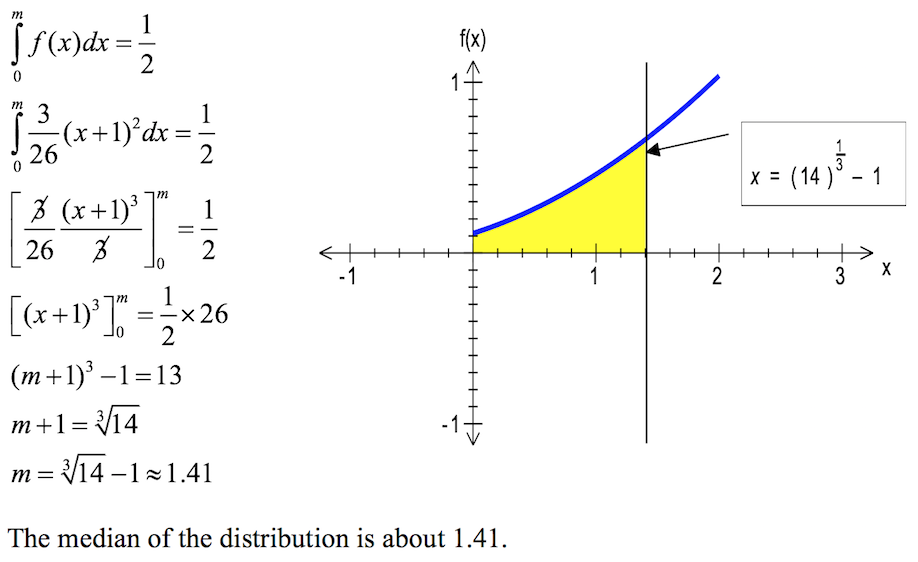
\includegraphics{mediancont.png}

The \textbf{mode} of a continuous r.v. \(X\) with a pdf \(f(x)\) is the
value of \(x\) for which \(f(x)\) takes a maximum value. Thus the mode
is the \(x\)-coordinate of the maximum point on the graph of \(f(x)\).

\emph{Hint}: To find \(x\) one need to solve for
\(\{x:f'(x)=0,f''(x)<0\}\) in cases of differentiable \(f\) and use
other turning point tests for \(f\) not differentiable at the turning
point.

\textbf{Solution}

 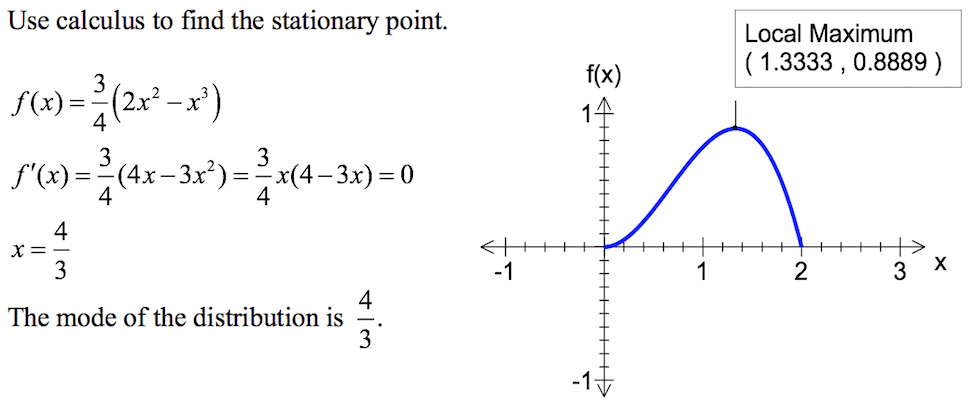
\includegraphics{modecont.png}

\end{frame}

\begin{frame}{Cumulative distribution functions}

\begin{itemize}
\item
  For a continuous random variable (r.v.) with probability density
  function \(f(x)\), the \textbf{cumulative distribution function}
  \(F(x)\) is defined as \(\mathbb{P}(X\le x)\).
\item
  Just as a cumulative probability mass function for a discrete random
  variable is obtained by summing all probabilities up to and including
  a given value, the cumulative density function involves integrating
  all probability density up to and including a point. This yields
  \[\mathbb{P}(X\le x)=F(x)=\int^x_{-\infty}f(t)dt\]
  \[\mathbb{P}(X\le x)=\mathbb{P}(X<x)\qquad\text{as}\,\,\mathbb{P}(X=x)=0\]
\item
  Similarly, if we know \(F(x)\), we can easily obtain \(f(x)\) since
  \(F(x)=\int^x_{-\infty}f(t)dt\) implies \(f(x)=\frac{dF(x)}{dx}\).
\end{itemize}

\end{frame}

\begin{frame}{Common continuous distribution}

\begin{itemize}
\item
  Uniform distribution
\item
  Triangular distribution
\item
  Exponential distribution
\item
  Beta distribution
\item
  Gamma distribution
\item
  Normal distribution
\end{itemize}

\end{frame}

\begin{frame}{Uniform Distribution}

\begin{itemize}
\item
  The simplest type of continuous distribution is \textbf{Uniform
  Distribution}.
\item
  This distribution is \textbf{rectangular in shape} and is defined by
  minimum and maximum values.
\item
  The probability density function is fixed over a continuous range from
  \(a\) to \(b\). This is sometimes denoted by \(U[a,b]\).
\item
  { Key characteristics }:

  \begin{itemize}
  \item
    Probability density function:
    \(f_X(x)=\begin{cases} \frac{1}{b-a}\quad a\le x\le b\\ 0\quad\text{ otherwise} \end{cases}\).
  \item
    Cumulative distribution function: \(F_X(x)=\frac{x-a}{b-a}\)
  \item
    Parameter constraints: \(a<b\)
  \item
    Mean: \(\frac{a+b}{2}\) \frenchspacing  variance:
    \(\frac{(b-a)^2}{12}\)
  \end{itemize}
\end{itemize}

\includegraphics{Lec5_files/figure-beamer/unnamed-chunk-1-1.pdf}

\end{frame}

\begin{frame}{Uniform Distribution: Example}

ACU provides shuttle bus service to students while they are on campus
every 10 mininutes between 7am til 9pm during weekdays. Students arrive
at the bus stop at random times. The time that a student waits is
uniformly distributed from 0 to 10 minutes.

\begin{enumerate}
\def\labelenumi{\arabic{enumi}.}
\tightlist
\item
  Draw a graph of this distribution
\end{enumerate}

\includegraphics{Lec5_files/figure-beamer/unnamed-chunk-2-1.pdf}

\begin{enumerate}
\def\labelenumi{\arabic{enumi}.}
\setcounter{enumi}{1}
\tightlist
\item
  Show that the area of this uniform distribution is 1.00.
\end{enumerate}

\begin{itemize}[<+->]
\tightlist
\item
  The times students must wait for the bus is uniform over the interval
  from 0 minutes to 10 minutes, so in this case \(a=0\) and \(b=10\).
  The area is (height)(base) \(\frac{1}{10-0}(10-0)=1\).
\end{itemize}

\begin{enumerate}
\def\labelenumi{\arabic{enumi}.}
\setcounter{enumi}{2}
\tightlist
\item
  How long will a student have to wait for a bus on average? In other
  words, what is the mean waiting time?
\end{enumerate}

\begin{itemize}[<+->]
\tightlist
\item
  \[\mu=\frac{a+b}{2}=\frac{0+10}{2}=5,\quad \sigma=\sqrt{\frac{(b-a)^2}{12}}=\sqrt{\frac{(10-0)^2}{12}}\]
\end{itemize}

\begin{enumerate}
\def\labelenumi{\arabic{enumi}.}
\setcounter{enumi}{3}
\tightlist
\item
  Let \(X\) be the waiting time in minutes. What is the probability a
  student will wait between 3 and 7 minutes?
\end{enumerate}

\begin{itemize}[<+->]
\item
  \begin{align*}
  \mathbb{P}(3<X<7)&=\underbrace{1/10}_{\text{height}}\times \underbrace{(7-3)}_{\text{base}}\\
  &=0.4
  \end{align*}
\end{itemize}

\end{frame}

\begin{frame}{Gamma distribution}

This distribution is often used to model insurance claim modelling. We
write \(X\sim\text{Gamma}(\alpha,\beta)\) to denote that we have a
random variable \(X\) that has a Gamma distribution with parameters
\(\alpha\) (scale) and \(\beta\) (rate.

\begin{itemize}
\item
  \textbf{probability density}:
  \(f_X(x)=\frac{\beta^{\alpha}}{\Gamma(\alpha)}x^{\alpha-1}e^{-\beta x}\)
  for \(x\ge 0\)
\item
  \textbf{Parameter constraints}: \(\alpha>0,\beta>0\)
\item
  \textbf{mean}: \(\frac{\alpha}{\beta}\) \textbf{variance}:
  \(\frac{\alpha}{\beta^2}\) \textbf{m.g.f.}:
  \(\left(\frac{\beta}{\beta-t}\right)^{\alpha}\), provided \(t<\beta\).
\end{itemize}

\includegraphics{Lec5_files/figure-beamer/unnamed-chunk-3-1.pdf}

\end{frame}

\begin{frame}{Exponential distribution: Special case of Gamma}

If we set \(\beta=\lambda\) and \(\alpha=1\), then we have
\(X\sim\text{Exp}(\lambda)\). The density becomes

Moreover, integrate the density function from \(0\) to \(\infty\), we
obtain the cumulative distribution function given as

\begin{align*}F_X(x)=\begin{cases} 1-e^{-\lambda x}\quad\forall\quad x\ge 0\\ 0\qquad\text{for}\,\,x< 0 \end{cases}
\end{align*}

One of the interesting properties of the exponential is the memoryless
property. (We will discuss this later on of the semester.)

\[\mathbb{E}X=\frac{1}{\lambda},\quad\text{Var}X=\frac{1}{\lambda^2}\]
One interesting properties of the exponential distribution is the
\emph{memoryless property}:

\begin{itemize}
\item
  Let \(W\sim \exp(\lambda)\) and consider two times a,b\textgreater{}0.
\item
  What is the chance that we need to wait a further \(b\) to see an
  arrival, given that we have already waited
  \(a\),i.e.\(\mathbb{P}(W>a+b|W>a)\)
\end{itemize}

\begin{align}
\mathbb{P}(W>a+b|W>a)&=\frac{\mathbb{P}(W>a+b,W>a)}{\mathbb{P}(W>a)}\\
&=\frac{\mathbb{P}(W>a+b)}{\mathbb{P}(W>a)}=\frac{\int^{\infty}_{a+b}\lambda e^{-\lambda x}dx}{\int^{\infty}_{a}\lambda e^{-\lambda x}}dx=\frac{e^{-\lambda(a+b)}}{e^{-\lambda a}}=e^{-\lambda b}\\&=\mathbb{P}(W>b)
\end{align}

\begin{itemize}
\item
  The distribution of future waiting times is independent of the times
  already waited
\item
  For example, if taxis arrive randomly, the chance you will wait a
  further 10 minutes is the same regardless of whether you have been
  waiting 30 minutes already or have just arrived!
\end{itemize}

\textbf{Exercise}

It has been determined over time that for a particular brand of magnetic
recording tape the distance \(X\) (in centimetres) between surface flaws
has the following probability density function
\[f_X(x)=\begin{cases} 0.02 e^{-0.02 x},\quad\text{for}\,\,x\ge 0\\ 0\quad\text{for}\,\,x< 0 \end{cases}\]
A flaw has been detected. What is the probability that another flaw will
be detected within the next metre?

\textbf{Solution}

Over \(1\) metre \(x=100cm\). We have

\begin{align*}
\mathbb{P}(0\le X\le 100)=F(100)-F(0)&=F(100)\\
&=\int^{100}_0 0.02 e^{-0.02 t}dt=[-e^{-0.02x}]^{100}_0\\
&=1-e^{-2}=0.8647\,\,\text{approximately.}
\end{align*}

\end{frame}

\begin{frame}[fragile]{Density of the Exponential Distribution with
\(\lambda=1,2,3,4\)}

\begin{Shaded}
\begin{Highlighting}[]
\KeywordTok{par}\NormalTok{(}\DataTypeTok{mfrow =} \KeywordTok{c}\NormalTok{(}\DecValTok{2}\NormalTok{,}\DecValTok{2}\NormalTok{))}
\KeywordTok{curve}\NormalTok{(}\KeywordTok{dexp}\NormalTok{(x, }\DecValTok{1}\NormalTok{), }\DecValTok{0}\NormalTok{, }\DecValTok{3}\NormalTok{, }\DataTypeTok{main =}\StringTok{"lambda = 1"}\NormalTok{)}
\KeywordTok{curve}\NormalTok{(}\KeywordTok{dexp}\NormalTok{(x, }\DecValTok{2}\NormalTok{), }\DecValTok{0}\NormalTok{, }\DecValTok{3}\NormalTok{, }\DataTypeTok{main =}\StringTok{"lambda = 2"}\NormalTok{) }
\KeywordTok{curve}\NormalTok{(}\KeywordTok{dexp}\NormalTok{(x, }\DecValTok{3}\NormalTok{), }\DecValTok{0}\NormalTok{, }\DecValTok{3}\NormalTok{, }\DataTypeTok{main =}\StringTok{"lambda = 3"}\NormalTok{) }
\KeywordTok{curve}\NormalTok{(}\KeywordTok{dexp}\NormalTok{(x, }\DecValTok{4}\NormalTok{), }\DecValTok{0}\NormalTok{, }\DecValTok{3}\NormalTok{, }\DataTypeTok{main =}\StringTok{"lambda = 4"}\NormalTok{)}
\end{Highlighting}
\end{Shaded}

\includegraphics{Lec5_files/figure-beamer/echo-1.pdf}

\end{frame}

\begin{frame}{Relation between Poisson and Exponential Distribution}

There exists a natural connection between Poisson and Exponential
distribution. If events occur on average at the rate of \(\lambda\) per
unit of time, then there will be on average \(\lambda t\) occurrences
per \(t\) units of time. The Poisson distribution describes this process
is therefore \(P(x)=e^{-\lambda t}\frac{(\lambda t)^x}{x!}\), from which
\(P(x=0)=e^{-\lambda t}\) is the probability of no occurences in \(t\)
units of time. Put it in another way, \(\mathbb{P}(x=0)=e^{-\lambda t}\)
is the probability that the time \(T\), to the first occurence is
greater than \(t\), i.e.
\[\mathbb{P}(T>t)=\mathbb{P}(x=0|\mu=\lambda t)=e^{-\lambda t}\]
Conversely, the probability that an event does occur during \(t\) units
of time is given by
\[\mathbb{P}(T\le t)=1-\mathbb{P}(x=0|\mu=\lambda t)=1-e^{-\lambda t}\]
Note that this is the cumulative exponential distribution which, when
differentiated with respect to \(t\), produces the probability density
function of the exponential distribution
\(f(t)=F'(t)=\lambda e^{-\lambda t}\).

\end{frame}

\begin{frame}{The normal (Gaussian) distribution}

\begin{itemize}
\tightlist
\item
  One of the most frequently used continuous probability distribution is
  the \emph{Normal distribution}. The normal distribution plays a very
  central role in mathematical statistics and the business/physical
  world. We use the notation \(X\sim N(\mu,\sigma^2)\) denotes a
  normally distributed random variable with mean \(\mu\) and variance
  \(\sigma^2\).
\end{itemize}

\includegraphics{Lec5_files/figure-beamer/unnamed-chunk-4-1.pdf}

\begin{itemize}
\item
  \textbf{density}:
  \(f_X(x)=\frac{1}{\sqrt{2\pi}\sigma}\exp\left(-\frac{1}{2}\left(\frac{x-\mu}{\sigma}\right)\right)\)
  for \(-\infty<x<\infty\)
\item
  \textbf{parameter constraints}: \(-\infty<\mu<\infty\), \(\sigma>0\).
\item
  \textbf{mean}: \(\mu\)
\item
  \textbf{variance}: \(\sigma^2\)
\end{itemize}

\end{frame}

\begin{frame}{The standard normal (Gaussian) distribution}

\begin{itemize}
\tightlist
\item
  Standard normal: When \(\mu=0\) and \(\sigma^2=1\), then we have a
  \emph{standard} normal random variable and we use \(Z\) to denote
  such, i.e. \(Z\sim N(0,1)\). The standard normal distribution is
  presented using the \(z\)-scores: \[Z=\frac{X-\mu}{\sigma}\] which is
  the number of standard deviation away from the mean.
\end{itemize}

\includegraphics{Lec5_files/figure-beamer/unnamed-chunk-5-1.pdf}

\end{frame}

\begin{frame}{The Standard normal distribution table}

\[\Phi(z)=\mathbb{P}(Z\le z)\] is used to denote the c.d.f. of a
standard normal distribution. For example, Let \(Z\sim N(0,1)\). Suppose
we want to find out the area up to 0.9, i.e. \[\mathbb{P}(Z\le 0.9)\]

\includegraphics{Lec5_files/figure-beamer/unnamed-chunk-6-1.pdf}

\begin{itemize}
\tightlist
\item
  Three methods are available.
\end{itemize}

\end{frame}

\begin{frame}{Method one: Integration}

\[\int^{0.9}_{-\infty}\frac{1}{\sqrt{2\pi}}e^{-\frac{y^2}{2}}dy\] (No
closed form!)

\end{frame}

\begin{frame}{Method two: Use table}

\includegraphics{zscore.png}

\end{frame}

\begin{frame}[fragile]{Method three: Use R}

The \texttt{pnorm(x)} command works out the lower tail area.

The \texttt{pnorm(x,lower.tail=F)} command works out the lower tail
area.

\begin{Shaded}
\begin{Highlighting}[]
\KeywordTok{pnorm}\NormalTok{(}\FloatTok{0.9}\NormalTok{)}
\end{Highlighting}
\end{Shaded}

\begin{verbatim}
## [1] 0.8159399
\end{verbatim}

\end{frame}

\begin{frame}[fragile]{Calculating probabilities using \(Z\)-scores}

The table usually gives values only for positive \(z_p\) but using the
symmetry property, one can easily derive for negative values. Note,
\[\Phi(-z):=\mathbb{P}(Z\le -z)=1-\mathbb{P}(Z\le z)=:1-\Phi(z)\] so
that for instance, \[\mathbb{P}(Z\le -0.9)=1-0.2118=0.1841\]

\begin{Shaded}
\begin{Highlighting}[]
\KeywordTok{pnorm}\NormalTok{(}\FloatTok{0.9}\NormalTok{)}
\end{Highlighting}
\end{Shaded}

\begin{verbatim}
## [1] 0.8159399
\end{verbatim}

\begin{Shaded}
\begin{Highlighting}[]
\KeywordTok{pnorm}\NormalTok{(}\FloatTok{0.3}\NormalTok{,}\DataTypeTok{lower.tail=}\NormalTok{F)}
\end{Highlighting}
\end{Shaded}

\begin{verbatim}
## [1] 0.3820886
\end{verbatim}

\begin{Shaded}
\begin{Highlighting}[]
\DecValTok{1}\OperatorTok{-}\KeywordTok{pnorm}\NormalTok{(}\FloatTok{0.3}\NormalTok{)}
\end{Highlighting}
\end{Shaded}

\begin{verbatim}
## [1] 0.3820886
\end{verbatim}

We can get probability values like

\begin{align}\mathbb{P}(-0.3\le Z\le 0.9)&=\Phi(0.9)-\Phi(-0.3)\,\,\text{use}\,\,\Phi(-z)=1-\Phi(z)\\
&=0.8159399-0.3820886= 0.4338513
\end{align}

\begin{Shaded}
\begin{Highlighting}[]
\FloatTok{0.8159399}\OperatorTok{-}\FloatTok{0.3820886}
\end{Highlighting}
\end{Shaded}

\begin{verbatim}
## [1] 0.4338513
\end{verbatim}

For non-standard normal distribution, we can always standardise using
the property that if \(X\sim N(\mu,\sigma^2)\), then
\[Z=\frac{X-\mu}{\sigma}\sim N(0,1)\] and
\[\mathbb{P}(X\le x)=\mathbb{P}\left(\frac{X-\mu}{\sigma}\le \frac{x-\mu}{\sigma} \right)=\mathbb{P}\left(Z\le \frac{x-\mu}{\sigma} \right)\]

Say, \(X\sim N(100,25)\), then the probability that \(X\) will be
between 92 and 112 is

\begin{align*}
\mathbb{P}(92\le X\le 112)
&=\mathbb{P}(\frac{92-100}{5}\le Z\le \frac{112-100}{5})\\
&=\Phi(2.4)-\Phi(-1.6)=0.9918-0.0548=0.9370
\end{align*}

\end{frame}

\begin{frame}[fragile]{Inverse standard normal: quantile}

In the previous slides we explained how to find the probability that a
value from a normal distribution will be less than some value, \(x\).

Now we wish to solve the inverse problem- given a probability, can we
such the value \(x\) such that there is this probability of being less.
These values are called \textbf{quantiles} of the distribution.

\textbf{Example}: The distribution of the weights of pink lady apples
arriving at a packhouse follows a normal distribution with \(\mu=180g\),
\(\sigma=10g\).Using the standard normal table, we can translate apple
weights \(x\), into \(Z\)-scores and uses the \(Z\)-scores to find the
probability of getting an apple with weight less than \(x\).

** The largest 10\% of apples will be sold for export. How large will
these apples be? **

To find the inverse standard normal, we follow

\[\text{Probability}\,\,\longrightarrow \,\,\text{z-score}\,\,\longrightarrow \,\,x\]

\begin{itemize}
\tightlist
\item
  Step 1: Using Rstudio,
\end{itemize}

\begin{Shaded}
\begin{Highlighting}[]
\KeywordTok{qnorm}\NormalTok{(}\FloatTok{0.8997}\NormalTok{)}
\end{Highlighting}
\end{Shaded}

\begin{verbatim}
## [1] 1.279844
\end{verbatim}

Alternatively, one can use the standard normal table

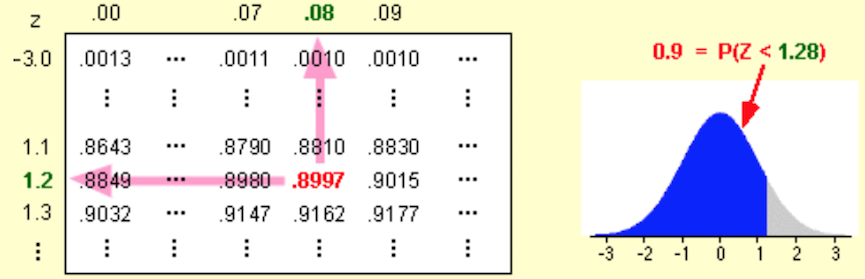
\includegraphics{quantile.png} The question essentially asks for weight
\(x\), such that \[\mathbb{P}(\text{weight}<x)=0.9\]

\begin{itemize}
\tightlist
\item
  Step 2. To get \(x\)-value from the \(Z\)-score we will use the
  following \[x=\mu+Z\sigma\]
\end{itemize}

(Remember the \(z\)-score tells us how much standard deviation.)

\end{frame}

\begin{frame}{Lognormal Distribution}

\begin{itemize}
\item
  In some applications-especially in financial problems - it proves
  useful to restrict to a distribution which is positive and skewed. One
  such useful case arises with the lognormal distribution.
\item
  In probability theory, a log-normal distribution is a continuous
  probability distribution of a random variable whose logarithm is
  normally distributed.
\item
  Thus, if the r.v. \(X\) is log-normally distributed, then
  \(Y=\text{ln}(X)\) has a normal distribution.
\item
  Consider \(X\sim \text{lognormal}(\mu,\sigma^2)\). The density is
  given as
  \[\frac{1}{x\sigma\sqrt{2\pi}}\exp\left[-\frac{1}{2}\left(\frac{\ln x-\mu}{\sigma}\right)\right],\quad x>0\]
\item
  Parameter constrains: \(-\infty<\mu<\infty,0<\sigma<\infty\)
  \[\mathbb{E}X=\exp\left(\mu+\frac{1}{2}\sigma^2\right)\]
  \[\text{var}X=e^{2\mu+\sigma^2}(e^{\sigma^2}-1)\] If
  \(Y\sim N(\mu,\sigma^2)\) and \(X=e^Y\), then \(X\) is lognormal; or
  \(\text{ln}X\sim N(\mu,\sigma^2)\).

  \begin{itemize}
  \tightlist
  \item
    \(X=\exp(Y)\sim\text{lognormal}(\mu,\sigma^2)\) is said to have a
    lognormal distribution with paramteters \(\mu\) and \(\sigma^2\).
  \end{itemize}
\end{itemize}

\includegraphics{Lec5_files/figure-beamer/unnamed-chunk-12-1.pdf}

\end{frame}

\begin{frame}[fragile]{Lognormal Distribution: Examples}

\begin{itemize}
\item
  Models of stock prices are often based on the lognormal distribution.
\item
  In actuarial science, the distribution is often used to model claim
  sizes.
\item
  Product of independent lognormal random variables are lognormal (think
  why?)
\item
  To calculate probabilities for a lognormal random variables, restate
  them as probabilities about the associated normal random variables.
\end{itemize}

\begin{align*}
\mathbb{P}(X\le a)&=\mathbb{P}(\text{ln}X\le\text{ln} a)\\
&=\mathbb{P}\left(\frac{\text{ln}X-\mu}{\sigma}\le\frac{\text{ln}a-\mu}{\sigma}\right)
\end{align*}

\begin{itemize}
\tightlist
\item
  \textbf{Exercise}
\end{itemize}

Losses from large fires can often be modelled using a lognormal
distribution.

Suppose that the average loss due to fire for building of a particular
type is \$25 million and the standard deviation of the loss is \$10
million.

Determine the probability that a large fire results in losses exceeding
\$40 million.

\textbf{Soln}:

\begin{align*}
\mathbb{P}(X> 40)&=1- \mathbb{P}(X\le 40)\\
&=1-\mathbb{P}(\text{ln}X\le\text{ln}40)\\
&=1-\left(\frac{\text{ln}X-\mu}{\sigma}\le \frac{\text{ln}40-\mu}{\sigma}\right)\\
&=\mathbb{P}(Z\le \frac{\text{ln}40-\mu}{\sigma})\\
&=\mathbb{P}(Z\le \frac{\text{ln}40-25}{10})
\end{align*}

\begin{Shaded}
\begin{Highlighting}[]
\NormalTok{(}\KeywordTok{log}\NormalTok{(}\DecValTok{40}\NormalTok{)}\OperatorTok{-}\DecValTok{25}\NormalTok{)}\OperatorTok{/}\DecValTok{10}
\end{Highlighting}
\end{Shaded}

\begin{verbatim}
## [1] -2.131112
\end{verbatim}

\begin{Shaded}
\begin{Highlighting}[]
\KeywordTok{pnorm}\NormalTok{(}\OperatorTok{-}\FloatTok{2.131112}\NormalTok{)}
\end{Highlighting}
\end{Shaded}

\begin{verbatim}
## [1] 0.01653996
\end{verbatim}

\end{frame}

\end{document}
